\chapter{Main Orientation Net}

\section{引言}
在上一章我们详细介绍了RSA算法,RSA用来解决基于BoW图像检索框架中的几何校验问题。这一章将介绍Main Orientation Net(MONet),MONet用来解决现有基于CNN图像检索框架中无法很好解决图片旋转的问题。本章首先介绍相关研究工作,确定需要解决的问题;然后逐步介绍MONet的模型结构、模型参数和训练方案等;最后介绍基于CNN的图像检索框架,并通过实验证明MONet确实可以解决所提出的问题。


\subsection{相关工作}
\begin{figure}
	\centering
	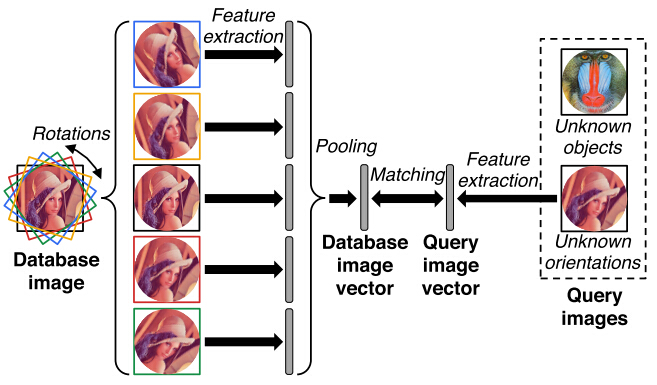
\includegraphics[width=\textwidth]{MaxPooling.jpg}
	\caption{使用MaxPooling解决图片旋转问题}\label{fig:maxpooling}
\end{figure}
在最初提出基于CNN的图像检索的工作\cite{babenko2014neural}中,对数据集中包含不同方向的图片做了两种简单的处理:
\begin{enumerate}
	\item 将所有图片旋转为正向;
	\item 或在训练时进行数据扩大,即将训练数据进行旋转($\pm90^{\circ}$)。
\end{enumerate}
以上两种方法虽然可以一定程度解决图片旋转的问题,但并不具有实用性。

\cite{chandrasekhar2015practical}提出了使用MaxPooling的方法,将不同方向的图片的特征进行融合,以达到对查询图片旋转的鲁棒性。\ref{fig:maxpooling}展示了使用MaxPooling融合图片特征并进行检索的过程。具体操作如下:
\begin{enumerate}
	\item 得到数据库图片的旋转的版本,旋转的范围为$-p^{\circ}$到$p^{\circ}$;
	\item 使用CNN网络得到所有图片(一张图片不同角度的副本)的特征;
	\item 使用MaxPooling将这些特征融合为一个特征,MaxPooling即保留这些特征向量每一维的最大值;
	\item 查询图片的处理和与数据图库片的相似度计算过程不变。
\end{enumerate}

通过CNN得到的图片特征是稀疏的,只有一些维度上有较大值:深度神经网络中对应节点产生的相应。正是由于CNN特征稀疏这一特点,才使得使用MaxPooling进行特征融合变为可能,MaxPooling保留了不同特征中的关键信息。虽然MaxPooling的方法可以很好的解决图片旋转的问题,但是其扩展性很差。第一,PCA降维方法不能与CNN特征结合使用;第二,该方案无法应用到传统的BoW图像检索框架中。在本章我们将提出不同的方案来解决图片旋转的问题,这种方法具有更好的扩展性,不影响原来的检索结构,也可以应用到传统的BoW框架中。

\section{图片方向}

\subsection{图片的梯度方向}
\begin{figure}
	\centering
	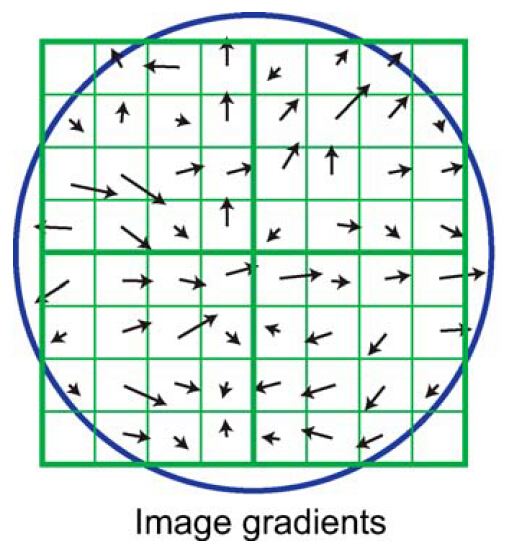
\includegraphics[width=0.5\textwidth]{gradient.jpg}
	\caption{图片区域梯度方向示意图}\label{fig:gradient}
\end{figure}
在介绍图片主方向之前,我们先介绍计算机视觉中经常遇到的一个相似的概念:图片的梯度方向。令$L(x,y)$表示一个像素的坐标,则图片的梯度方向由相邻像素之间的梯度大小$m(x,y)$和方向$\theta(x,y)$共同决定:
\begin{equation}
m(x,y) = \sqrt{(L(x+1,y)-L(x-1,y))^2 + L(x,y+1)-L(x,y-1))^2}
\end{equation}
\begin{equation}
\theta(x,y)=\tan^{-1}\frac{L(x,y+1) - L(x,y-1)}{L(x+1,y) - L(x-1,y)}
\end{equation}

图\ref{fig:gradient}为一个图片区域的梯度方向示意图。梯度方向有很多应用,比如构建具有旋转不变性的描述符\cite{lowe2004distinctive}。但是,我们却无法用梯度方向来描述一幅图像的方向。这是由于在一副自然图片中,梯度方向的分布是接近均匀分布的,这一点也可以从图\ref{fig:RSA_dis_2}(c)中得到。所梯度方向往往应用于一块blob区域。

\subsection{图片的主方向}
由于拍摄时选取的角度问题,或者是人为修改,在进行图片检索时,查询图片(包括数据库图片)可能不是竖直的。而图片旋转会为图像检索带来不小的困难,在使用几何校验算法时由甚\cite{jegou2008hamming}\cite{lazebnik2006beyond}。在使用CNN的图像检索框架时,由于CNN提取的是图片的全局特征,图片旋转的问题将更为突出。为此,我们训练了一个学习图片主方向的网络Main Orientation Net(MONet)。

\begin{figure}
	\centering
	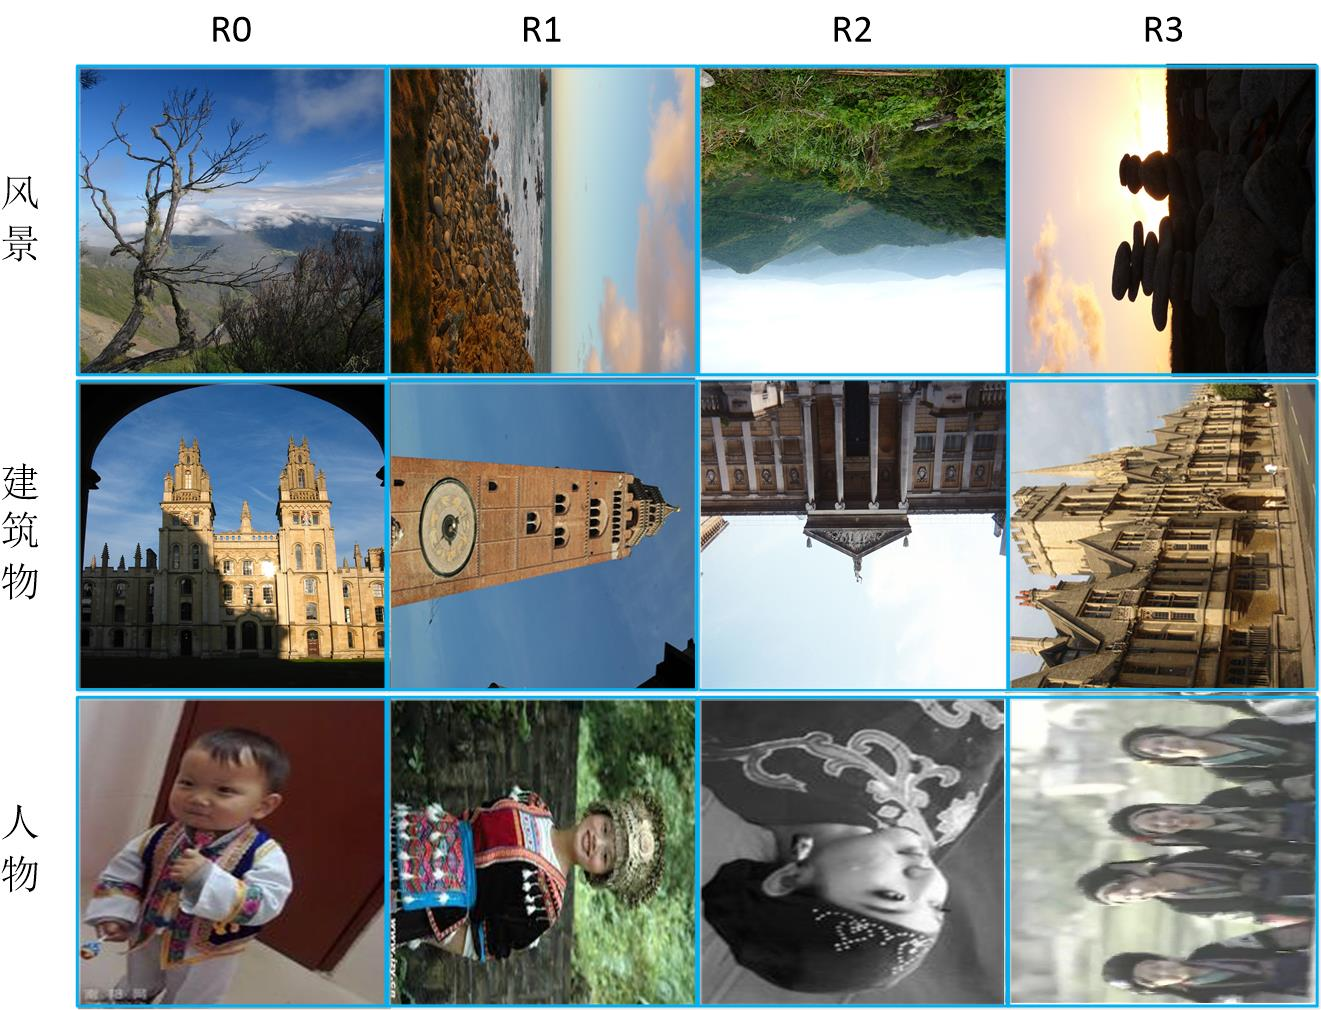
\includegraphics[width=0.8\textwidth]{Main_Orientation.jpg}
	\caption{不同主方向的自然图片}\label{fig:main_ori}
\end{figure}

我们定义图片的主方向为图片中垂直于地表的方向,为了简化问题,我们认为在图像检索中图片只存在4中方向,即$0^{\circ}$、$90^{\circ}$、$180^{\circ}$和$270^{\circ}$,分别表示为$R0$,$R1$,$R2$和$R3$。图\ref{fig:main_ori}给出了风景、建筑物和人物在不同主方向下的情况。对于图\ref{fig:main_ori}中的情况,人很容易判断图片的主方向,我们希望MONet同样可以判断出图片的主方向。

\begin{figure}
	\centering
	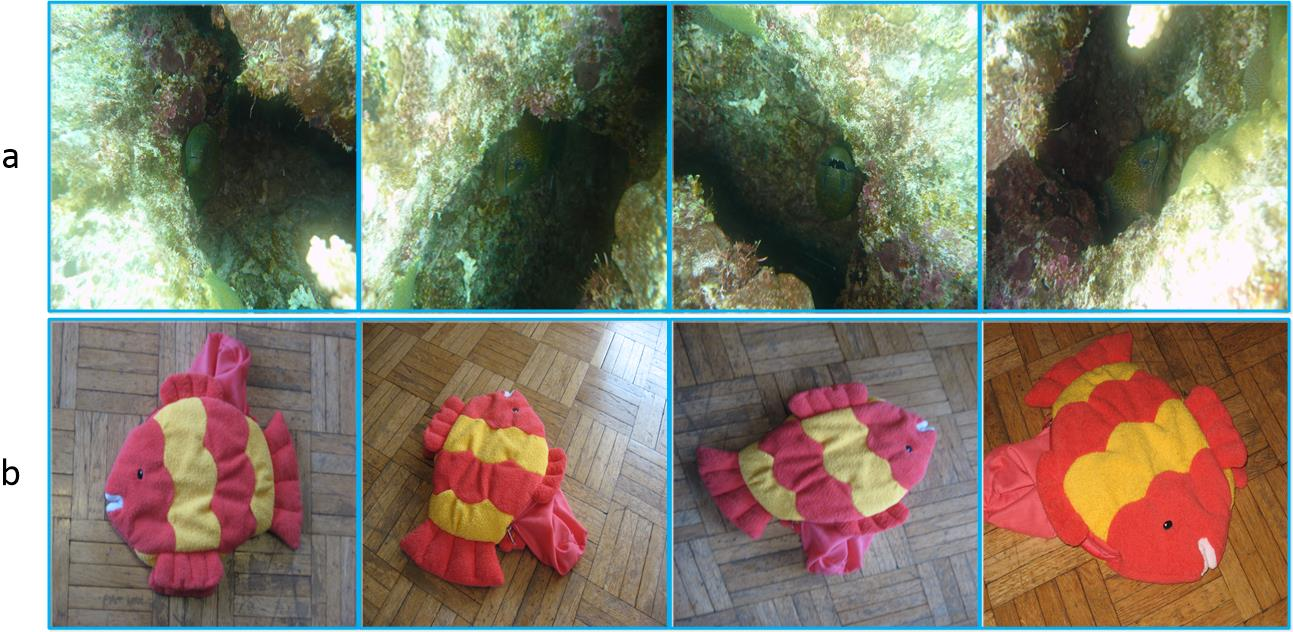
\includegraphics[width=0.8\textwidth]{None_MO.jpg}
	\caption{不容易确定主方向的自然图片}\label{fig:n_mo}
\end{figure}

在有些情况下,图片的主方向是不容易确定的。如图\ref{fig:n_mo}所示,其中(a)中的鱼不明显,所以很难判断图片的主方向;(b)中图片的方向并不重要,可以认为没有主方向。对于以上情况,MONet也是不予考虑的。

\section{图片主方向对检索的影响}
\begin{figure}
	\centering
	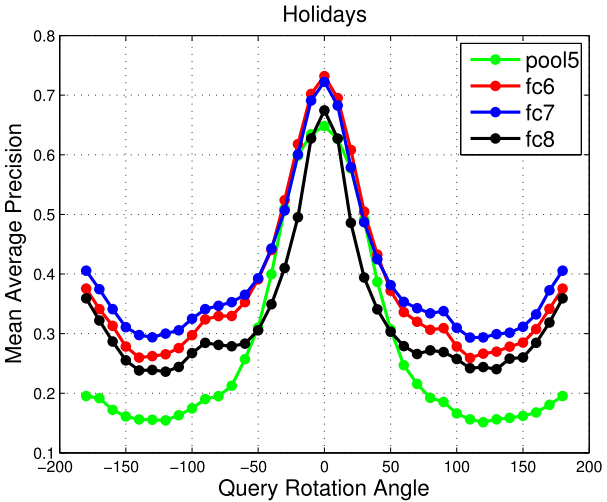
\includegraphics[width=0.7\textwidth]{Holidays_r.jpg}
	\caption{查询图片旋转对CNN检索框架的影响}\label{fig:hr}
\end{figure}
为了测试图片旋转对基于CNN的图像检索框架的影响,我们使用了2.3节介绍的框架进行旋转情况下的图像检索实验。图\ref{fig:hr}显示了不同旋转角度下的查询结果,其中横轴表示查询图片旋转的角度(从$-180^{\circ}$到$+180^{\circ}$),纵轴表示检索结果(用mAP表示),不同的曲线表示使用不同层的CNN特征。通过实验结果可以看出,查询图片的旋转对检索精度有很大的影响,当图片旋转$10^{\circ}$时,mAP就有明显的下降。可以想象,网络上存在的大量的经过旋转的图片将会对CNN图像检索框架产生严重的影响。

\section{MONet网络设计}
在设计MONet时,我们主要考虑了以下几点问题:
\begin{enumerate}
	\item MONet学习图片的主方向,而不关注图片的细节,所以该网络应该有更小的图片输入和更大的卷积核;
	\item 网络应该具有稀疏性,提高训练速度并减少参数量;
	\item 可以从MONet中方便的提取特征,用于后续处理;
	\item 在应用MONet时,可以快速的判断图片的主方向,保证图片检索的速度。
\end{enumerate}

我们借鉴了GoogLeNet中Inception\cite{szegedy2015going}的思想,设计了MONet的模型如图\ref{fig:monet_f}所示。其中,虚线框出的结构就是一个Inception\cite{szegedy2015going},Inception用稠密的网络结构模拟了稀疏网络结构,减少了参数量的同时提高了运行速度,并且Inception还完成的多尺度的识别,保证了模型的识别能力。

\begin{figure}
	\centering
	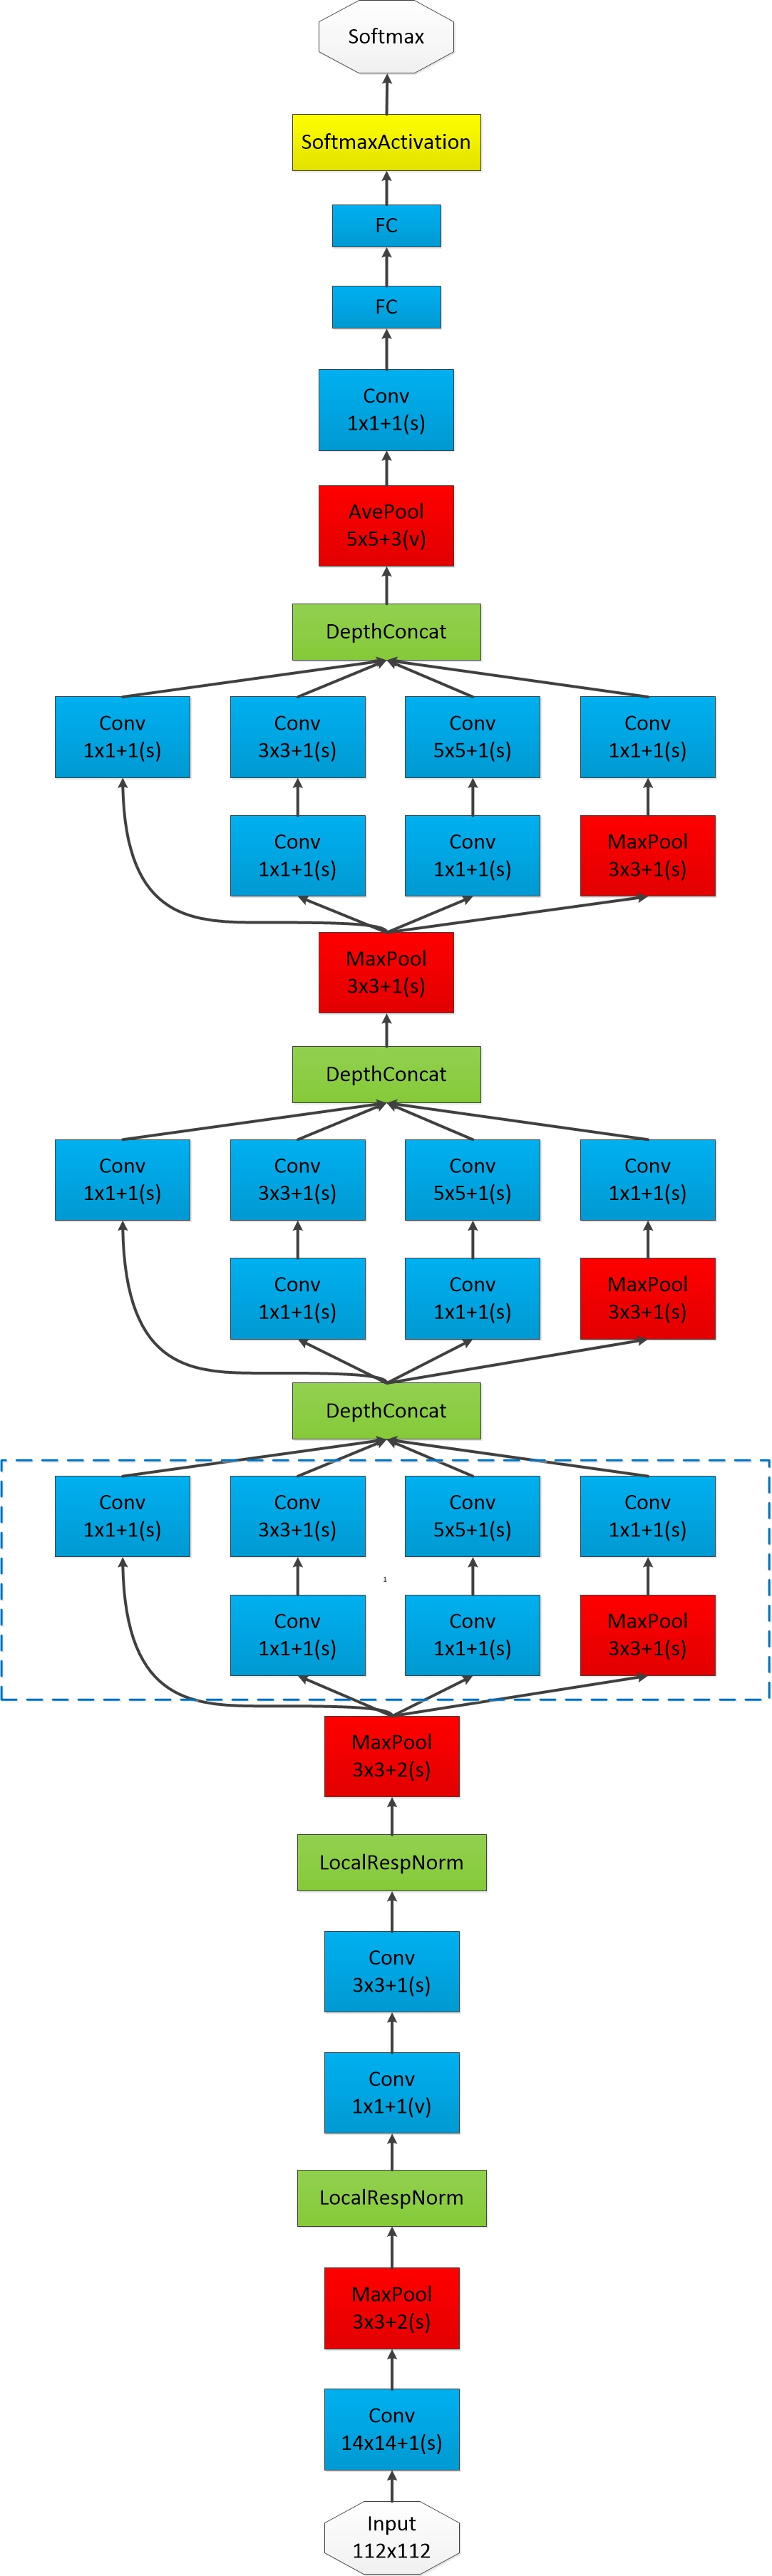
\includegraphics[width=0.43\textwidth]{MONet_frame.jpg}
	\caption{MONet框架图}\label{fig:monet_f}
\end{figure}

表\ref{tab:monet}列出了MONet各层的参数。其中,$x\times x$ reduce表示在进行$x\times x$卷积前进行的削参操作,pool proj表示在进行pooling操作之前进行的投影操作,目的是减少feature map的个数。
\begin{table}
	\begin{center}
		\begin{tabular}{|c|c|c|c|c|c|c|c|c|}
			\hline
			type & patch size & $1\times1$ & $3\times3$ & $3\times3$ & $5\times5$ & $5\times5$ & pool & params \\
			     & /stride    &            & reduce     &            &            &     reduce & proj &        \\
			\hline
			\hline
			conv & $14\times14/1$ & & & & & & & 11K\\
			\hline
			max  & $3\times3/2$ & & & & & & & \\
			\hline
			conv & $3\times3/1$ & & 64 & 192 & & & & 112K\\
			\hline
			max  & $3\times3/2$ & & & & & & &\\
			\hline
			incep(a) & & 64 & 96 & 128 & 16 & 32 & 32 & 159K\\
			\hline
			incep(b) & & 128 & 128 & 192 & 32 & 96 & 64 & 380K\\
			\hline
			max  & $3\times3/2$ & & & & & & &\\
			\hline
			incep(c) & & 192 & 96 & 208 & 16 & 48 & 64& 364K\\
			\hline
			ave & $5\times5/3$ & & & & & & &\\
			\hline
			fc(a) & & & & & & & & 8M\\
			\hline
			fc(b) & & & & & & & & 4K\\
			\hline
		\end{tabular}
	\end{center}
	\caption{MONet各层参数}
	\label{tab:monet}
\end{table}


\section{MONet网络训练}
由于训练数据有限,我们假设图片只有四个主方向,即$R0$,$R1$,$R2$和$R3$。这种假设也是合理的,因为在实际的图片库中,绝大多数的图片只有这四种主方向,而不会出现任意方向的旋转。为了保证MONet的可扩展性,我们在不同的数据集上进行训练和测试,同时这两个数据集最好有一定的相关性。所以在我们的实验中,我们用Paris\cite{philbin2008lost}上进行训练,在Oxford5K\cite{philbin2007object}进行测试。我们将图片主方向的学习过程认为是图片分类问题,具体流程如下:
\begin{enumerate}
	\item 图片预处理:分别将Paris和Oxford5K中的图片进行旋转,旋转后的角度($Rx$)即为图片的标签;
	\item 使用GoogLeNet在ILSVRC上的训练结果作为MONet的权重初值;
	\item 配置网络结构,并使用Paris进行训练(相当于fine-tune);
	\item 使用Oxford5K测试网络的性能;
	\item 后处理:包括PCA降维和SVM分类等。
\end{enumerate}

我们将batch大小设为32张图片,每500次迭代进行一次测试,两万次的迭代的结果如图\ref{fig:monet_t}所示,其中横轴为迭代次数,纵轴为准确率。可以看出当迭代2000次时,MONet的准确率基本达到峰值,我们将迭代两千次的网络作为后续试验的基本模型。

\begin{figure}
	\centering
	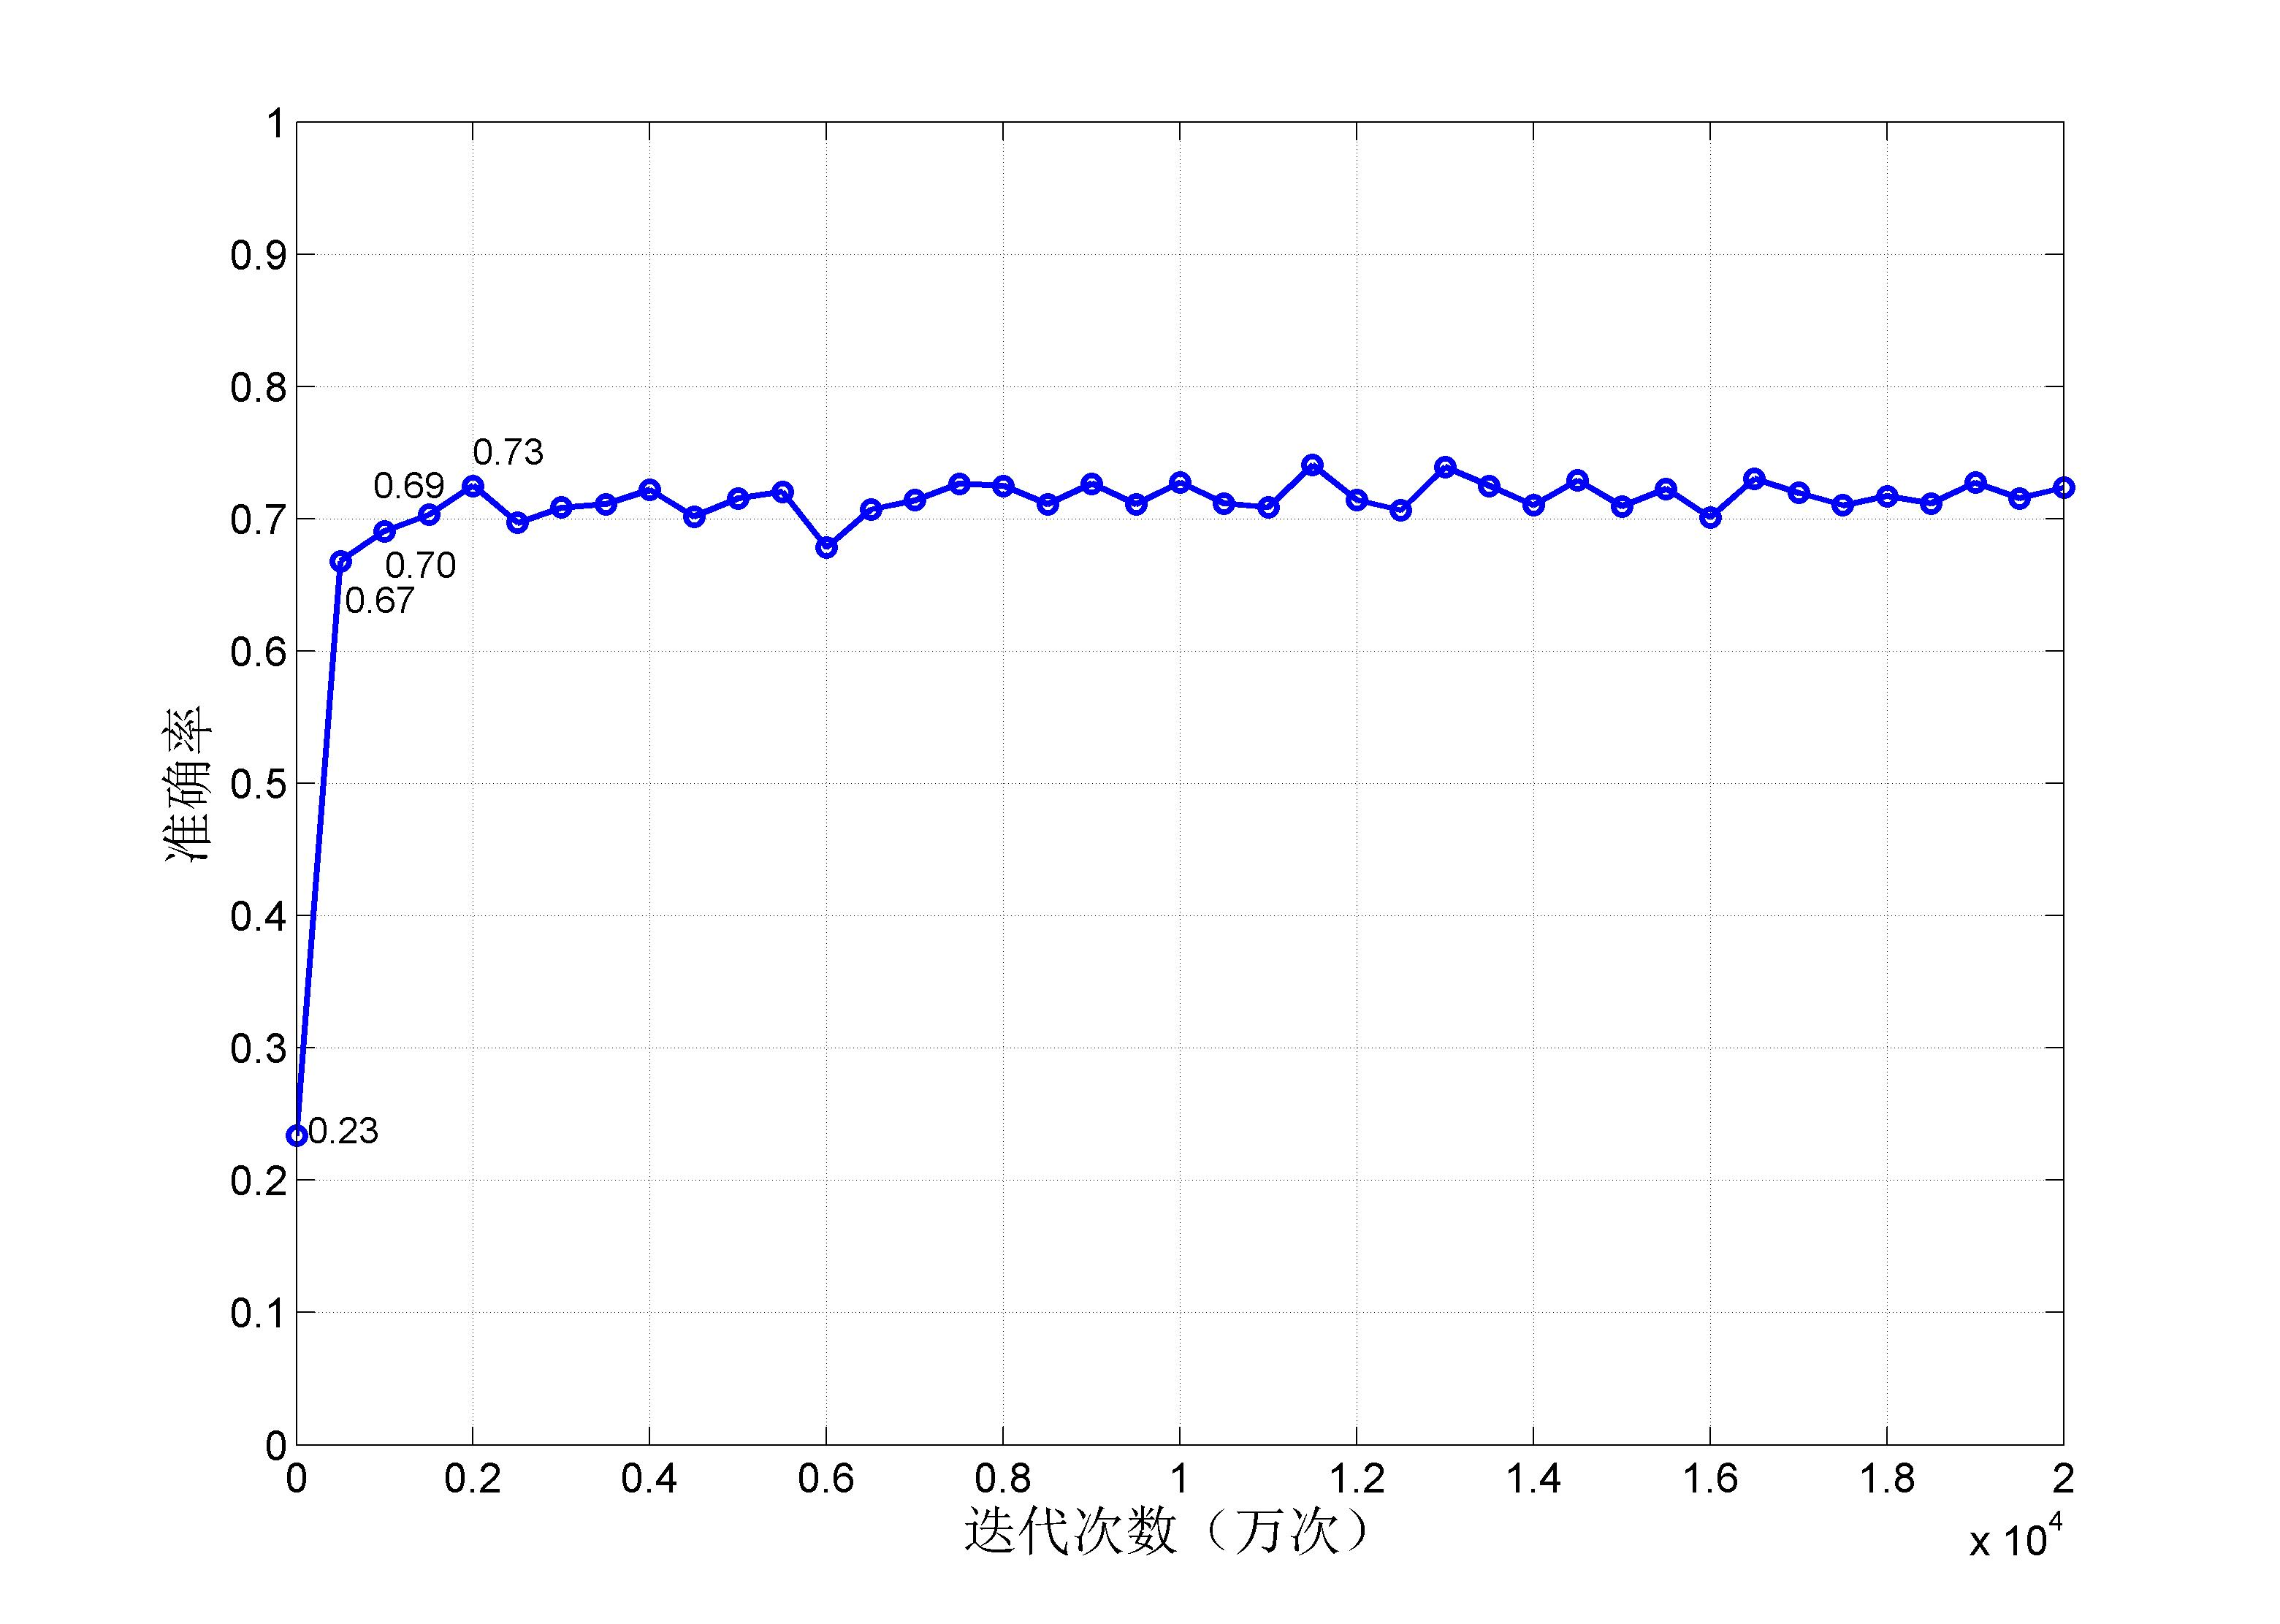
\includegraphics[width=0.7\textwidth]{MONet_train.jpg}
	\caption{MONet训练过程中的准确率变化情况}\label{fig:monet_t}
\end{figure}

为了进一步提高MONet的分类准确率,我们在MONet之后增加了一个SVM分类器。SVM分类器的输入为Paris图片的CNN特征(fc(a)层输出,1024维)和图片的主方向($Rx$),训练数据为Oxford5K的CNN特征。在添加SVM分类器后,MONet的准确率提高到0.810。最终,MONet的正整体结构如图\ref{fig:monet_ff}所示。

\begin{figure}
	\centering
	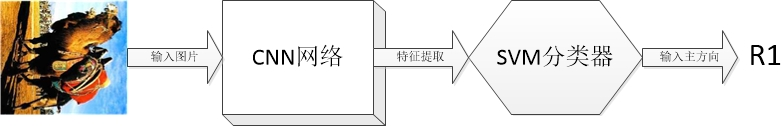
\includegraphics[width=0.9\textwidth]{MONet_frame_f.jpg}
	\caption{MONet整体结构}\label{fig:monet_ff}
\end{figure}

\section{CNN图像检索框架}
使用MONet进行图片检索是非常容易的,只需要将MONet作为查询图片的预处理步骤即可。这也是MONet的优点之一,可以方便的与现有的图像检索模型融合。使用CNN网络的图片检索整体框架如图\ref{fig:cnn_rf}所示,第一个CNN网络为MONet,用来判断图片的主方向;第二个CNN网络用于提取图片特征,完成相似度计算。

\begin{figure}
	\centering
	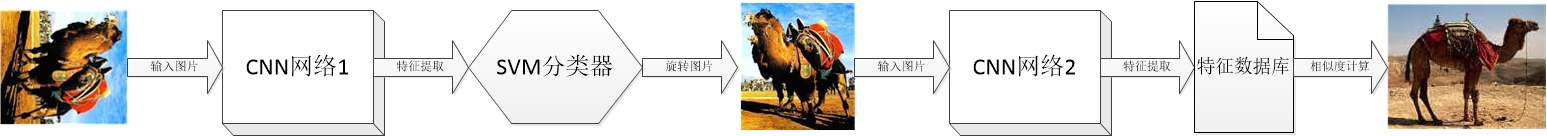
\includegraphics[width=\textwidth]{CNN_retrieval_frame.jpg}
	\caption{基于CNN的图像检索整体框架}\label{fig:cnn_rf}
\end{figure}

\section{实验}
我们针对相似图像检索任务对MONet的效果进行了测试。

\subsection{实验模型}
我们的实验模型主要由两部分组成,包括用于判断图片主方向的MONet和提取图片特征的AlexNet。模型整体框架如图\ref{fig:cnn_rf}所示。Baseline模型为不使用MONet进行处理的AlexNet,改进模型为经过旋转预处理的MONet,其实验结果分别标记为“AlexNet”和“MONet”。

\subsection{实验数据}
与训练MONet一样,我们进行测试时同样使用了Paris\cite{philbin2008lost}训练MONet,使用Oxford 5K\cite{philbin2007object}测试检索的性能。这主要是考虑了Paris和Oxford5K之间的相关性,即这两个数据库都只包含了建筑物,并且没有交集。Oxford数据集中的图片都是竖直的($R0$),因此我们将每个查询图片都生成4张不同主方向的图片,分别表示为$R0$、$R1$、$R2$和$R3$,并测试在不同主方向下的检索结果。

\subsection{图片特征}
在检索时,我们提取图片的四种特征,分别为AlexNet的Pooling 5层特征(9216维)、fully connected 6层特征(4096维)、fully connected 7层特征(4096维)和输出层特征(1000维)。图片的这些特征分别简记为“pool5”、“fc6”、“fc7”和“fc8”。

\subsection{实验结果}
\begin{figure}
	\centering
	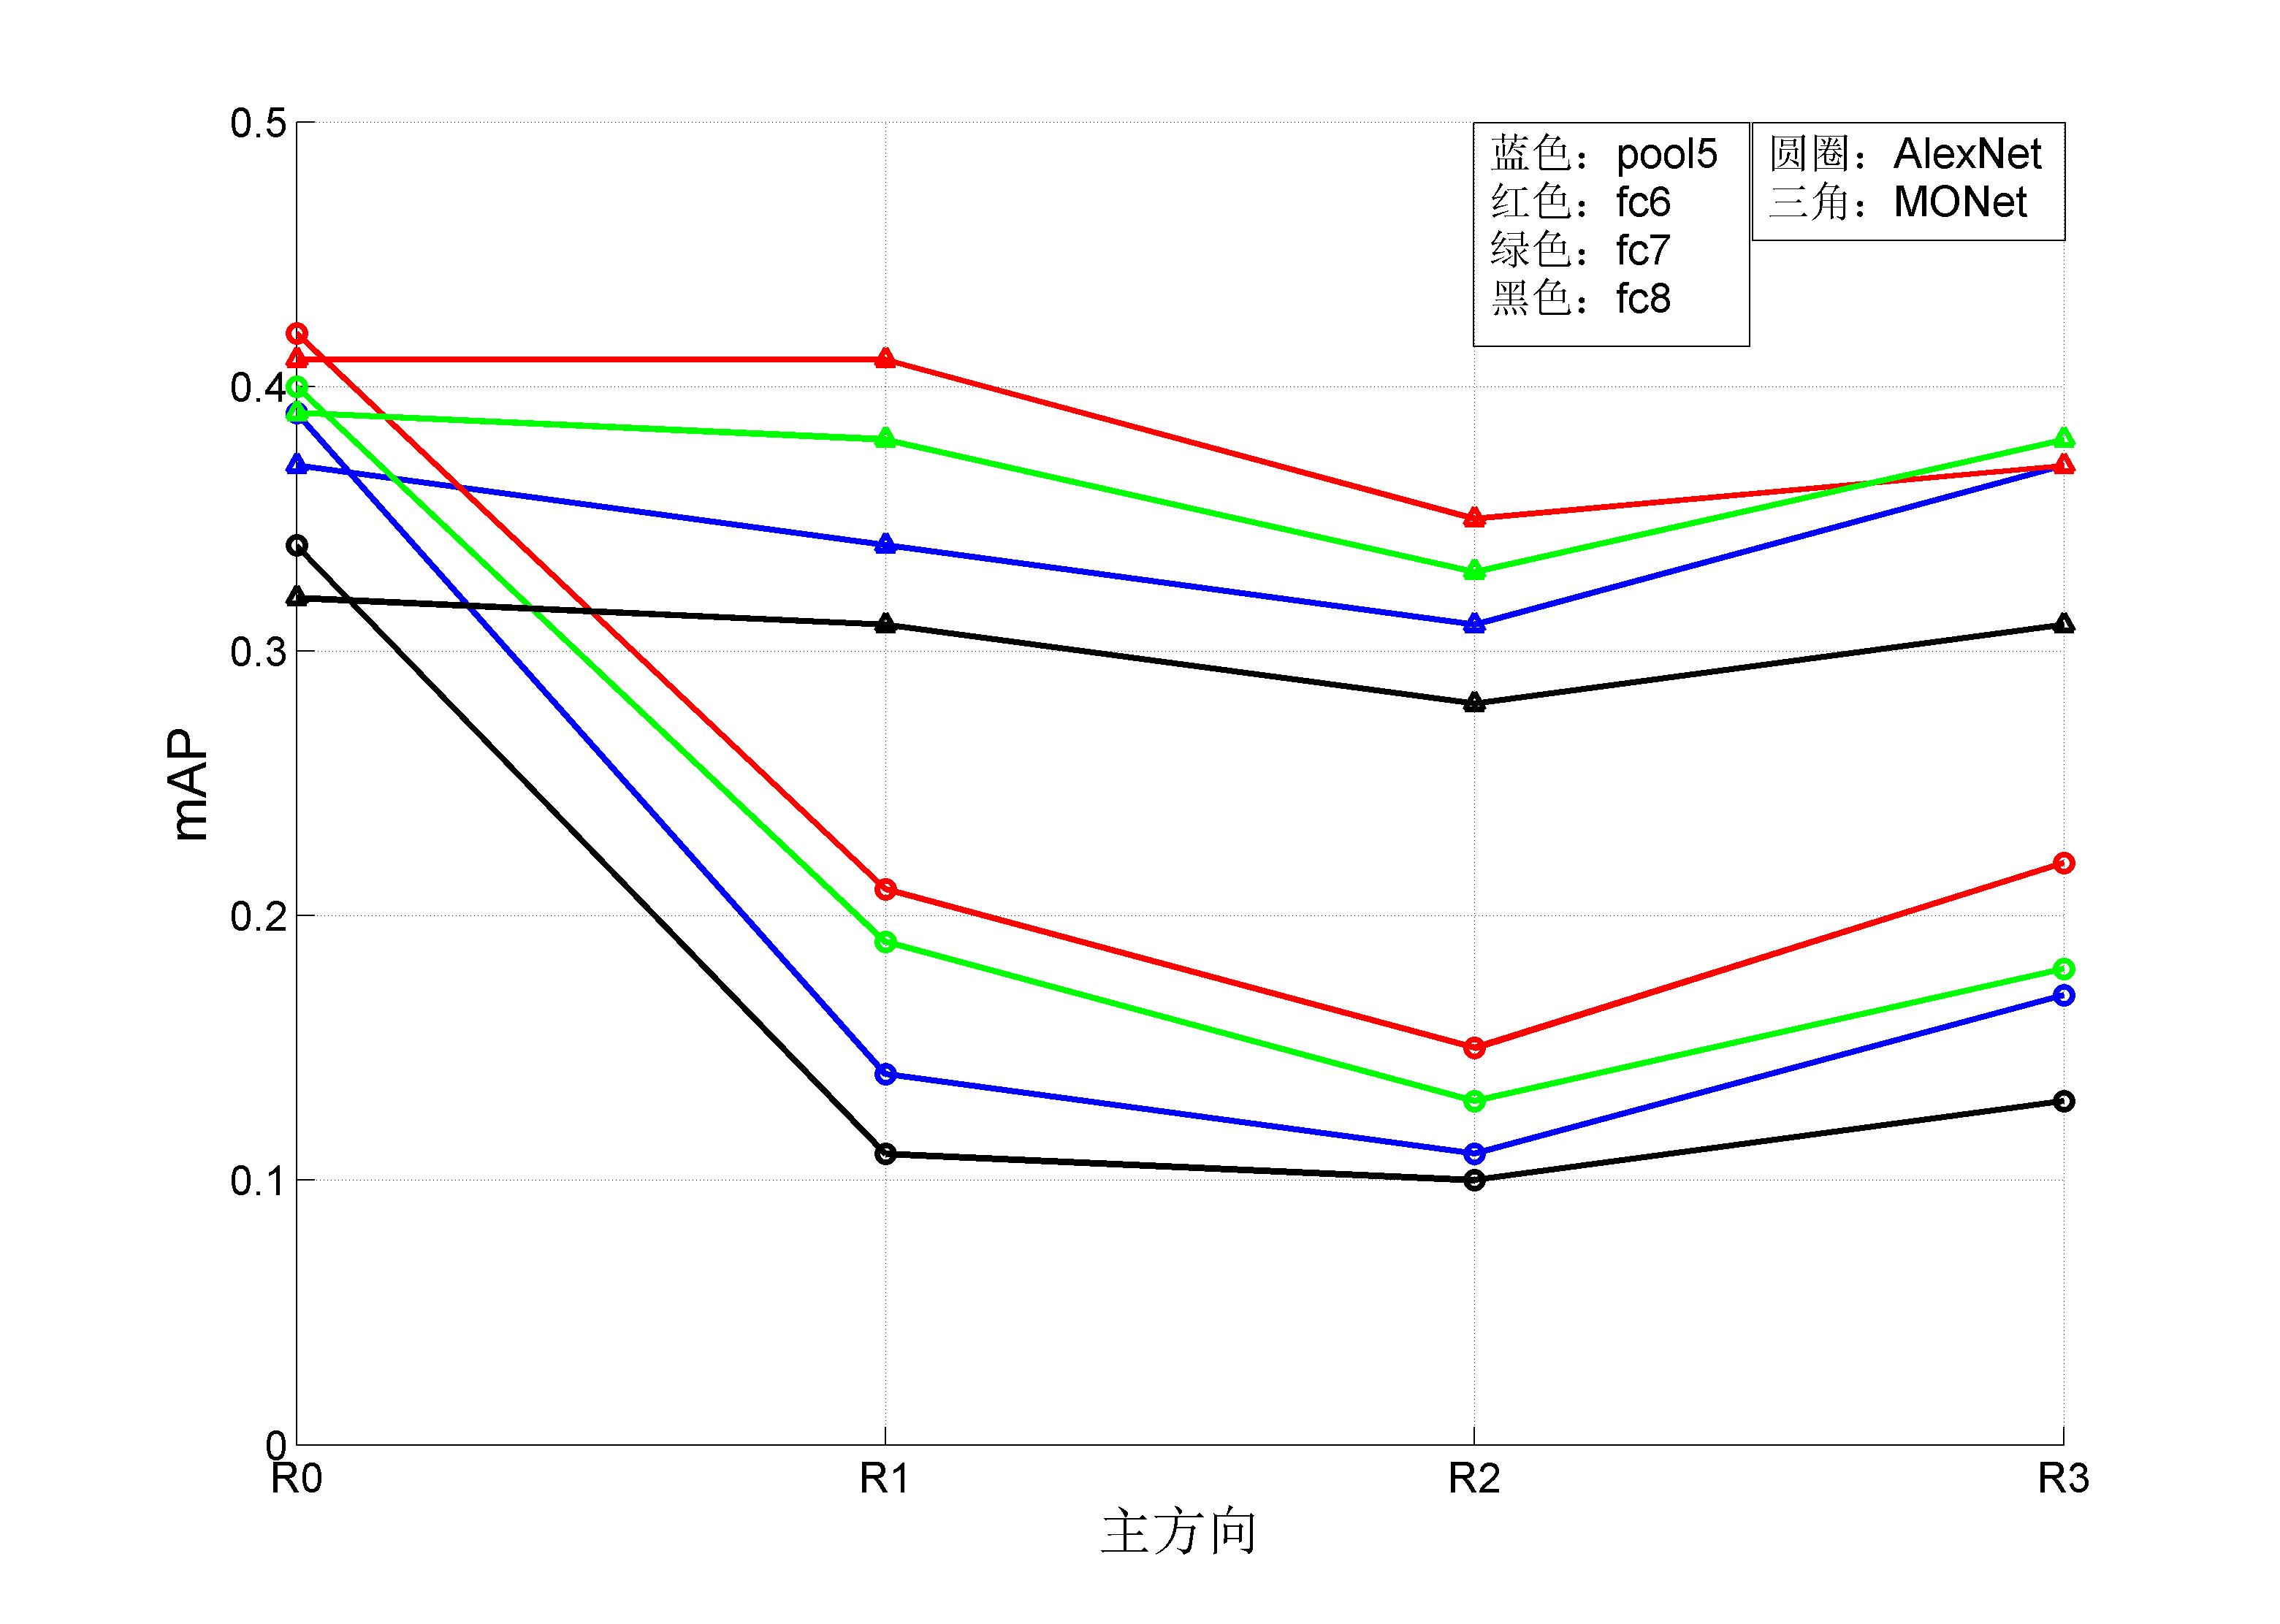
\includegraphics[width=0.8\textwidth]{MONet_res.jpg}
	\caption{MONet在Oxford5K数据集上的检索结果}\label{fig:monet_r}
\end{figure}
实验结果如图\ref{fig:monet_r}所示。其中,不同颜色的曲线表示使用AlexNet网络中不同层的特征,圆圈表示没有进行MONet预处理,三角表示进行MONet预处理后的结果。从图\ref{fig:monet_r}中可以看出,在图片旋转时,AlexNet网络的检索性能会显著下降,而经过MONet的预处理后,可以保证不同主方向的图片都可以有较好的检索结果。


\section{MONet的应用}
MONet对图片进行预处理,所以这个网络可以应用于任何的图片预处理步骤,本节就介绍MONet的两个应用。

\subsection{BoW框架下MONet的应用}
由于局部特征一般具有旋转不变性(例如SIFT\cite{lowe2004distinctive}),所以基于BoW框架的图像检索可以很好的应对图片旋转的问题。但是,正如2.5节中提到的现有的很多几何校验算法无法解决图片旋转的问题:\cite{philbin2007object}中的FSM和\cite{lazebnik2006beyond}中的SPM要求图片必须是竖直的;\cite{jegou2008hamming}中的WGC需要图片方向的先验知识。图片主方向的问题限制了很多几何校验算法的应用场景,而MONet可以很好的解决这个问题。

为了验证MONet对传统的BoW框架中的几何校验有帮助,我们做了如下对比实验:
\begin{enumerate}
	\item 使用经典的BoW框架和FSM\cite{philbin2007object}几何校验作为baseline,记作$R0$;
	\item 将查询图片进行$90^{\circ}$、$180^{\circ}$和$270^{\circ}$的旋转,并进行上述相同的实验,记作$R1$、$R2$和$R3$;
	\item 将查询图片进行$90^{\circ}$、$180^{\circ}$和$270^{\circ}$的\textbf{随机}旋转,并使用MONet进行预处理,再进行上述实验,记作MONet。
\end{enumerate}

通过上述实验设置,我们得到了表\ref{tab:monet_bow}的结果,其中每行表示Oxford5K中的一类建筑物,每列为不同的旋转和方法,结果为相应建筑物检索的mAP。通过表\ref{tab:monet_bow}可以看出,虽然BoW框架对图像的旋转有一定的鲁棒性,但是几何校验一般需要假设图片的主方向,所以当查询图片旋转时,检索精度有一定的下降;通过MONet的预处理(将超过80\%的图片旋转为正向),可以得到与不进行旋转情况相近的结果。通过以上结果可以得出结论,MONet可以与传统的BoW框架结合使用,使其更加对图片旋转更加鲁棒。
\begin{table}
	\begin{center}
		\begin{tabular}{|c|c|c|c|c|c|}
			\hline
						& $R0$  & $R1$ & $R2$ & $R3$ & MoNet \\
			\hline
			all\_souls	& 79.75 & 68.60 & 68.57 & 68.05 & 78.03\\
			\hline
			ashmolean   & 63.89 & 45.44 & 46.23 & 46.03 & 64.33\\
			\hline
			balliol     & 77.79 & 78.15 & 77.50 & 77.95 & 77.09\\
			\hline
			bodleian    & 90.61 & 79.55 & 79.62 & 80.41 & 91.44\\
			\hline
			christ\_church&64.91 & 60.91& 61.03 & 60.99 & 64.82\\
			\hline
			cornmarket  & 65.87 & 47.13 & 45.86 & 46.69 & 64.63\\
			\hline
			hertford    & 88.34 & 84.35 & 84.84 & 85.32 & 88.29\\
			\hline
			keble       & 93.70 & 83.69 & 83.80 & 83.98 & 94.04\\
			\hline
			magdalen    & 29.71 & 24.04 & 24.07 & 24.84 & 29.83\\
			\hline
			pitt\_rivers& 100.0 & 97.77 & 97.55 & 97.37 & 100.0\\
			\hline
			radcliffe\_camera& 77.41 & 74.38 & 74.27 & 73.69 &76.88\\
			\hline
			mAP         & 75.63 & 67.63 & 67.57 & 67.75 & 75.40\\
			\hline
		\end{tabular}
	\end{center}
	\caption{MONet与传统BoW框架结合的检索结果}
	\label{tab:monet_bow}
\end{table}

\subsection{服饰检测中MONet的应用}

基于MONet和CNN分类网络,我们设计了一个服饰检测系统,CostumeNet。CostumeNet用来识别图片中人物所穿服饰所属的民族。首先我们收集了两个数据集,用来测试和训练CostumeNet,分别为Costume-12和Costume-38。

\subsubsection{Costume-12数据集}
Costume-12为从网络上下载的12个中国少数民族服饰的数据集。这12个少数民族包括:白族、布依族、朝鲜族、傣族、俄罗斯族、回族、满族、蒙古族、苗族、维族、彝族和藏族。每一类包含约300张图片,共3635张图片。由于这些图片全部来自网络,可能存在错误,即图片中不包含相应类别的服饰,或服饰类别错误。绝大多数图片中包含人,即人穿着相应的民族服饰,部分图片可能是衣服、首饰甚至漫画。图\ref{fig:costume-12}展示了Costume-12中的部分图片。

\begin{figure}
	\centering
	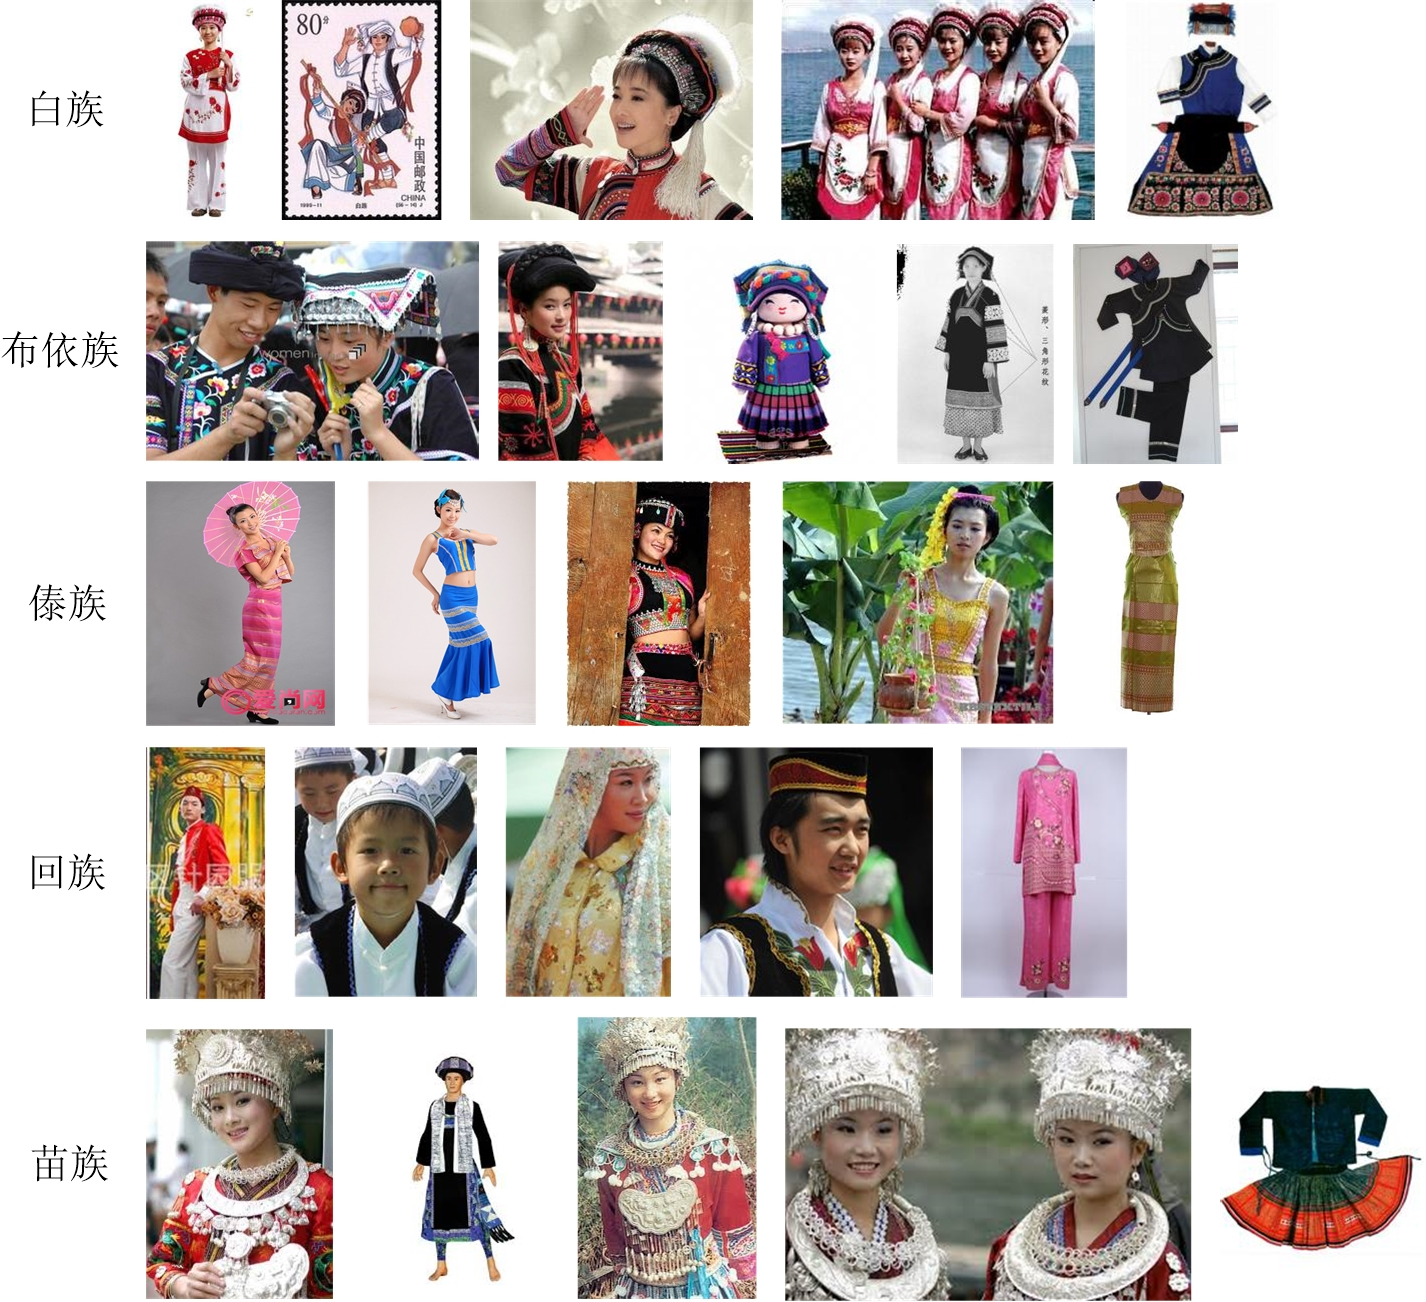
\includegraphics[width=1\textwidth]{costume-12.jpg}
	\caption{Costume-12数据集中的部分图片}\label{fig:costume-12}
\end{figure}

\subsubsection{Costume-38数据集}
Costume-38数据集包含38个中国少数民族,其图片来源于纪录片《中国少数民族》中的视频截图,因此图片中包含的服饰一定为相应民族的服饰,不会存在错误。由于每个民族的纪录片长度不同,所以得到的截图数量也不尽相同,多的有六十几张,少的只有二十张,共1342张图片。Costume-38数据集中绝大多数图片包含人,少部分图片只包含服饰、首饰等。图\ref{fig:costume-38}展示了Costume-38中的部分图片。

\begin{figure}
	\centering
	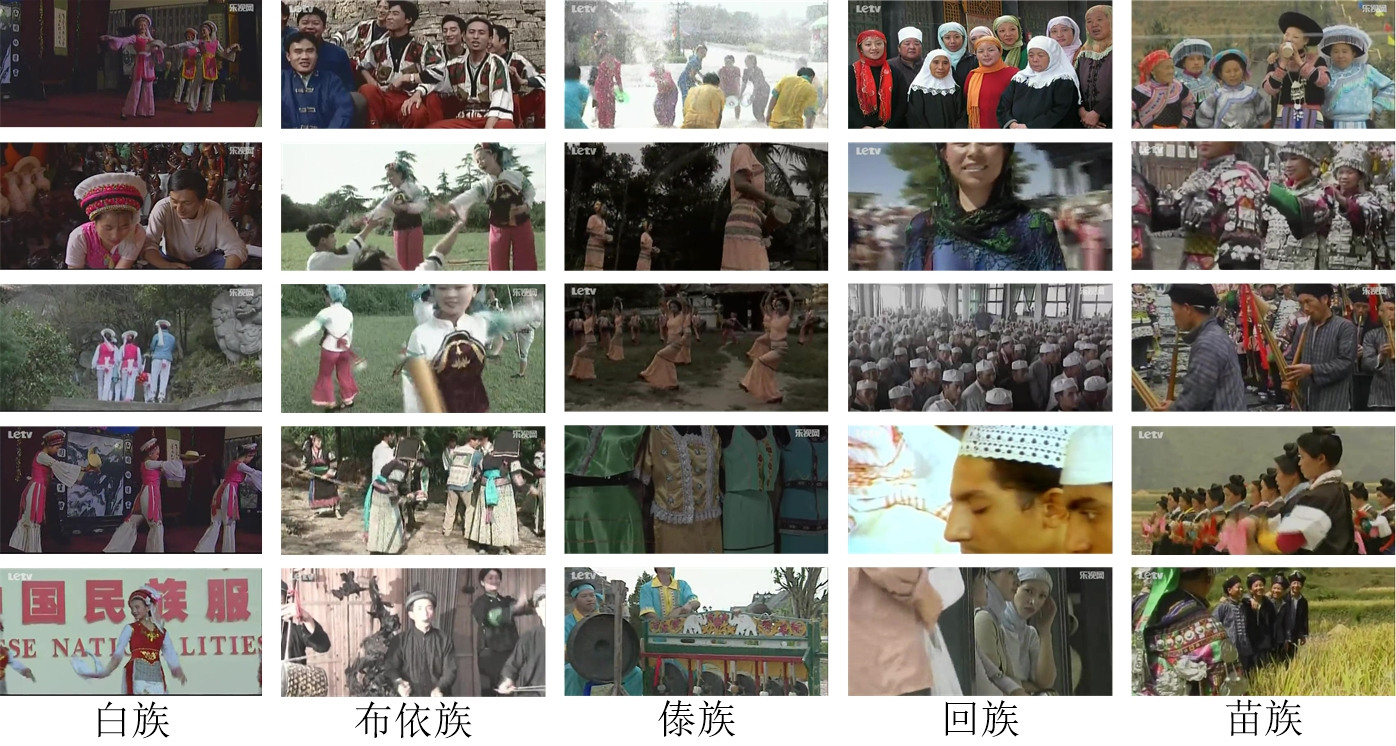
\includegraphics[width=1\textwidth]{costume-38.jpg}
	\caption{Costume-38数据集中的部分图片}\label{fig:costume-38}
\end{figure}

\subsubsection{实验流程与实验结果}

使用CostumeNet做服饰检测的流程与前面的MONet和使用CNN进行图像检索的思路类似,分为三个部分:
\begin{enumerate}
	\item 预处理:使用MONet判断图片的主方向;
	\item 训练和分类:使用预处理得到的图片训练VGG-19网络,并使用该网络对图片进行分类(Costume-12为12类,Costume-38为38类);
	\item 后处理:提取网络全连接层的输出作为图片的特征,使用SVM再进行分类。
\end{enumerate}

实验结果如表\ref{tab:costume}所示。其中第一列“SVM”表示使用VGG网络提取图片特征(不经过fine-tune)然后使用SVM分类的结果;第二列“VGG”表示使用VGG fine-tune的结果;第三列表示使用fine-tune的网络提取图片特征然后用SVM分类的结果;结果用准确率$R$表示($R=\frac{\#correct}{\#correct+\#false}$)。对于Costume-12数据集,每一类我们使用50张图片进行测试,其余图片进行训练;对于Costume-38数据集,每一类我们使用10张图片记性测试,其余图片进行训练。通过实验结果可以看出,直接使用未经过fine-tune的网络提取的特征做SVM效果并不理想,而使用fine-tune后的结果有较大的提升。使用“VGG+SVM”的策略,在Costume-12上可以达到95.3\%的准确率,在Costume-38上可以达到85.0\%的准确率,达到了较为理想的效果。并且在Costume-12数据集上,由于存在错误图片,准确率很难再有提升;而在Costume-38数据集上,每一类的图片数量有限,在后面的工作中,可以继续扩大数据集,提高准确率。
\begin{table}
	\begin{center}
		\begin{tabular}{|c|c|c|c|}
			\hline
			           & SVM & VGG & VGG+SVM \\
			\hline
			Costume-12 & 0.648 & 0.823 & 0.953\\
			\hline
			Costume-38 & 0.371 & 0.584 &0.850\\
			\hline
		\end{tabular}
	\end{center}
	\caption{CostumeNet实验结果}
	\label{tab:costume}
\end{table}

\subsubsection{Demo展示}
基于上述实验框架和模型,我们搭建了一个可以进行服饰检测的平台,其展示效果图\ref{fig:costume-demo}所示。
\begin{figure}
	\centering
	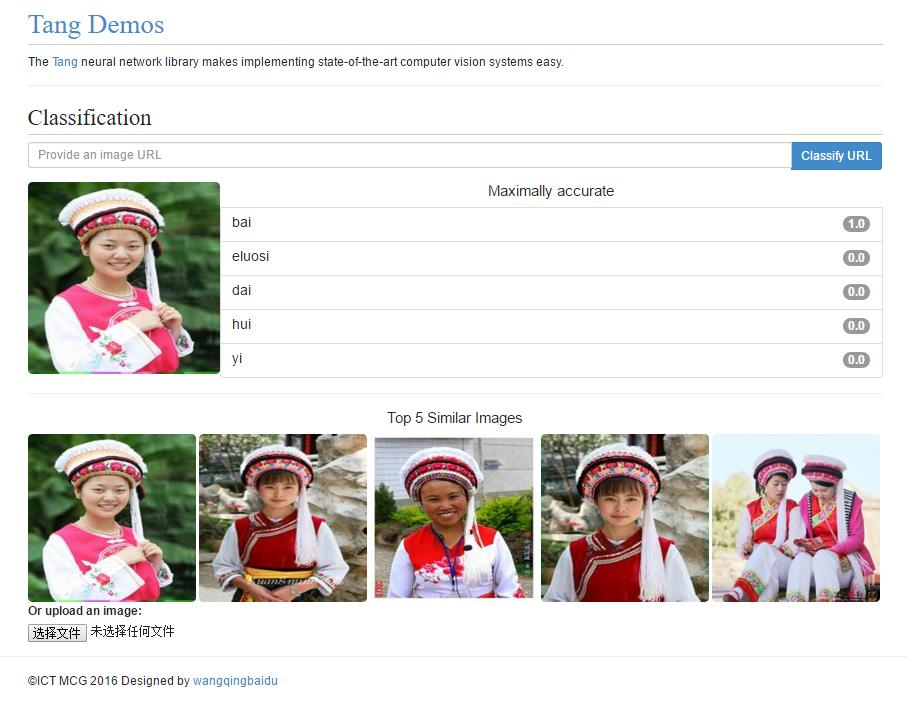
\includegraphics[width=1\textwidth]{cnndemo.jpg}
	\caption{服饰检测Demo展示}\label{fig:costume-demo}
\end{figure}


\section{本章小节}
在本章中,我们分析并证明了CNN图像检测框架中存在的一个问题:无法克服图片旋转带来的性能下降。我们也介绍了目前解决该问题的主流方法,包括数据扩大、Max Pooling特征融合等等,但是这些方法都有其局限性。通过分析以上问题,我们提出了MONet,其思想是通过学习的方向,训练出一个可以自动识别图片主方向的网络,并在进行图像检索之前通过MONet对图片记性预处理。在设计MONet时,我们考虑模型复杂度和训练、分类速度等问题,最终基于Inception思想设计出了MONet的网络结构。由于MONet是一个对图片的预处理步骤,所以可以简单地与现有的任何模型进行融合,本章也介绍了MONet的应用,包括将MONet应用于传统的基于BoW的检索框架和民族服饰检索任务。目前MONet也存在一些局限性,包括无法更加精细的判断图片的主方向;增加图像检索的预处理时间等。







